\documentclass[conference]{IEEEtran}
\IEEEoverridecommandlockouts
\usepackage{cite}
\usepackage{amsmath,amssymb,amsfonts}
\usepackage{algorithmic}
\usepackage{graphicx}
\usepackage{textcomp}
\usepackage{xcolor}
\usepackage{booktabs}
\usepackage{tabularx}
\usepackage{xurl}
\usepackage{placeins}

\def\BibTeX{{\rm B\kern-.05em{\sc i\kern-.025em b}\kern-.08em
    T\kern-.1667em\lower.7ex\hbox{E}\kern-.125emX}}

\begin{document}

\title{Rogue Wi-Fi Access Point Detector}

\author{
\IEEEauthorblockN{Tashfin Shakeer Rhythm}
\IEEEauthorblockA{2431079 \\
\textit{Department of Computer Science and Engineering} \\
\textit{Independent University, Bangladesh}\\
Dhaka, Bangladesh \\
2431079@iub.edu.bd}
\and
\IEEEauthorblockN{Md. Yalid Iqbal}
\IEEEauthorblockA{2420812 \\
\textit{Department of Computer Science and Engineering} \\
\textit{Independent University, Bangladesh}\\
Dhaka, Bangladesh \\
2420812@iub.edu.bd}
\and
\IEEEauthorblockN{Md. Boktier Ahmed Sojib}
\IEEEauthorblockA{2420947 \\
\textit{Department of Computer Science and Engineering} \\
\textit{Independent University, Bangladesh}\\
Dhaka, Bangladesh \\
2420947@iub.edu.bd}
\and
\IEEEauthorblockN{Wazid Abdullah}
\IEEEauthorblockA{2420290 \\
\textit{Department of Computer Science and Engineering} \\
\textit{Independent University, Bangladesh}\\
Dhaka, Bangladesh \\
2420290@iub.edu.bd}
\and
\IEEEauthorblockN{S M Amimul Ihsan}
\IEEEauthorblockA{2420845 \\
\textit{Department of Computer Science and Engineering} \\
\textit{Independent University, Bangladesh}\\
Dhaka, Bangladesh \\
2420845@iub.edu.bd}
}

\maketitle

\begin{abstract}
This paper presents a hardware-integrated Rogue Wi-Fi Access Point Detector and NAPT Repeater built on the ESP32-C6 RISC-V microcontroller \cite{esp32c6}, operating under the SoftAP SSID \texttt{Scarlet ESP32-C6}. The system provides six main operating modes: promiscuous packet sniffing, targeted AP ping monitoring, real-time data traffic monitoring, station MAC address logging, Denial-of-Service (DoS) flood detection, multi-port TCP honeypots (FTP, SSH, HTTP, HTTPS), and an automated Layer-3 Network Address and Port Translation (NAPT) Wi-Fi repeater \cite{napt_ref}. A non-blocking state machine manages user inputs through a single push button alongside an SSD1306 OLED display \cite{ssd1306}, status LEDs, an addressable RGB LED \cite{neopixel}, and a passive buzzer. System testing confirms fast packet inspection, quick honeypot connection handling, RSSI-based open network selection, and stable packet routing during threat alarms.
\end{abstract}

\begin{IEEEkeywords}
ESP32-C6, Rogue Access Point Detection, Wireless Intrusion Detection, Promiscuous Sniffing, Embedded Honeypot, Network Address and Port Translation (NAPT), Wi-Fi Repeater, IoT Security.
\end{IEEEkeywords}

\section{Introduction}
Wireless local area networks built on IEEE 802.11 standards \cite{ieee80211} connect many embedded IoT devices to local networks. Because Wi-Fi signals broadcast over an open medium, network nodes can be exposed to packet eavesdropping, MAC address spoofing, traffic floods, and port scanning. Enterprise networks defend against these threats using dedicated intrusion detection systems and server-based honeypots. However, field technicians and portable setups often lack a low-cost, portable tool that can monitor local Wi-Fi security while extending network range.

The ESP32-C6 microcontroller provides a practical platform for low-power security tools. Featuring a 32-bit RISC-V core with 2.4\,GHz Wi-Fi 6 (802.11ax) support \cite{esp32c6}, it includes promiscuous packet capture APIs \cite{espressif_idf} and an integrated LwIP TCP/IP stack \cite{lwip}. This enables a single board to inspect Wi-Fi packets, host basic TCP honeypots, and bridge client network traffic.

This paper presents the \textbf{Rogue Wi-Fi Access Point Detector} (\texttt{Scarlet ESP32-C6}), a portable hardware security monitor and Wi-Fi range extender. As shown in the system block diagram in Fig.~\ref{fig:block_diagram}, the ESP32-C6 acts as the main controller. It receives user inputs from a physical push button and displays real-time status updates across an SSD1306 OLED screen, indicator LEDs, an onboard addressable RGB LED, and a passive buzzer while communicating with local SoftAP clients and upstream access points.

% Project Block Diagram
\begin{figure}[htbp]
  \centering
  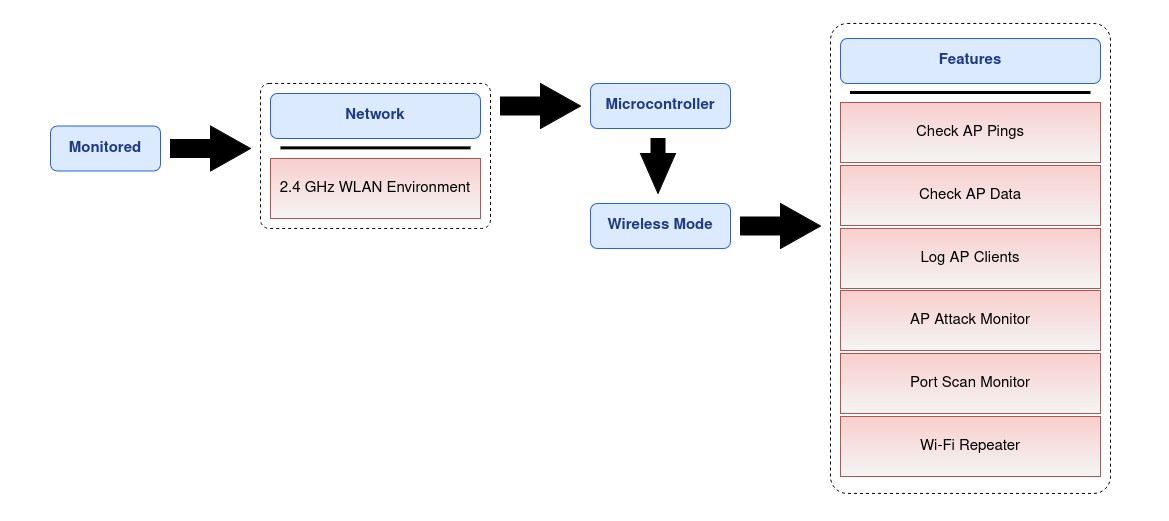
\includegraphics[width=\columnwidth]{block_diagram.png}
  \caption{Block diagram of the proposed system.}
  \label{fig:block_diagram}
\end{figure}

\section{Related Work}
Embedded Wi-Fi security projects often use custom firmware on ESP8266 or ESP32 microcontrollers for packet capture or access point spoofing \cite{espressif_idf}. However, existing open-source projects (such as ESP32 Marauder \cite{marauder}) primarily focus on packet sniffing and injection without offering network repeating, honeypot detection, or audio/visual hardware alerts. Commercial tools like the WiFi Pineapple \cite{pineapple} offer extensive features but run on a full Linux operating system, which increases hardware cost (~100--250\,USD), boot time (~45\,s), and power consumption. Microcontroller honeypots remain uncommon due to RAM constraints \cite{honeypot_iot}, and embedded Wi-Fi repeaters generally operate at Layer 2 without active security auditing \cite{napt_ref}.

The proposed Rogue Wi-Fi AP Detector combines Wi-Fi packet sniffing, multi-port TCP honeypots, station MAC logging, and Layer-3 NAPT routing into a single low-cost ESP32-C6 project under 12\,USD.

\section{Problem Statement}
Portable wireless security tools often present four practical limitations:
\begin{enumerate}
    \item \textbf{Single-Task Focus:} Most portable security devices perform frame sniffing or AP spoofing in isolation, lacking network bridging or honeypot capabilities.
    \item \textbf{High Operating Overhead:} Linux-based auditing platforms require significant startup time and power, limiting fast field deployment.
    \item \textbf{Lack of Local Physical Alerts:} Threat alerts are frequently sent only to remote web dashboards, providing no immediate acoustic or visual feedback to technicians on-site.
    \item \textbf{Unsecured Range Extension:} Standard micro-repeaters extend signals without auditing connected client traffic or automatically selecting strong open networks.
\end{enumerate}

\section{Methodology}

\subsection{System Overview \& Control Architecture}
The hardware setup consists of an ESP32-C6 microcontroller \cite{esp32c6}, an SSD1306 $128 \times 64$ I2C OLED display \cite{ssd1306}, a passive buzzer, two status LEDs (Blue for activity, Orange for warnings), an onboard WS2812 RGB LED \cite{neopixel}, and a push button.

As shown in the system architecture diagram in Fig.~\ref{fig:system_architecture}, the firmware uses a non-blocking button state machine to detect single clicks, double clicks, and long presses ($\ge 1000\,\text{ms}$). The button input changes menu items and switches operational modes. Table~\ref{tab:control_ui} details the button gesture timing.

\begin{table}[htbp]
\caption{System Button Interface Control Architecture}
\label{tab:control_ui}
\centering
\small
\begin{tabularx}{\linewidth}{@{}lcX@{}}
\toprule
\textbf{User Action} & \textbf{Timing} & \textbf{System Response} \\
\midrule
Single Click & $<400\,\text{ms}$ & Cycles menu selection (F1 $\rightarrow$ F6) \\
Double Click & $<300\,\text{ms}$ gap & Exit active mode to main menu \\
Long Press & $\ge 1000\,\text{ms}$ & Executes highlighted menu feature \\
\bottomrule
\end{tabularx}
\end{table}

% System Architecture Diagram
\begin{figure}[htbp]
  \centering
  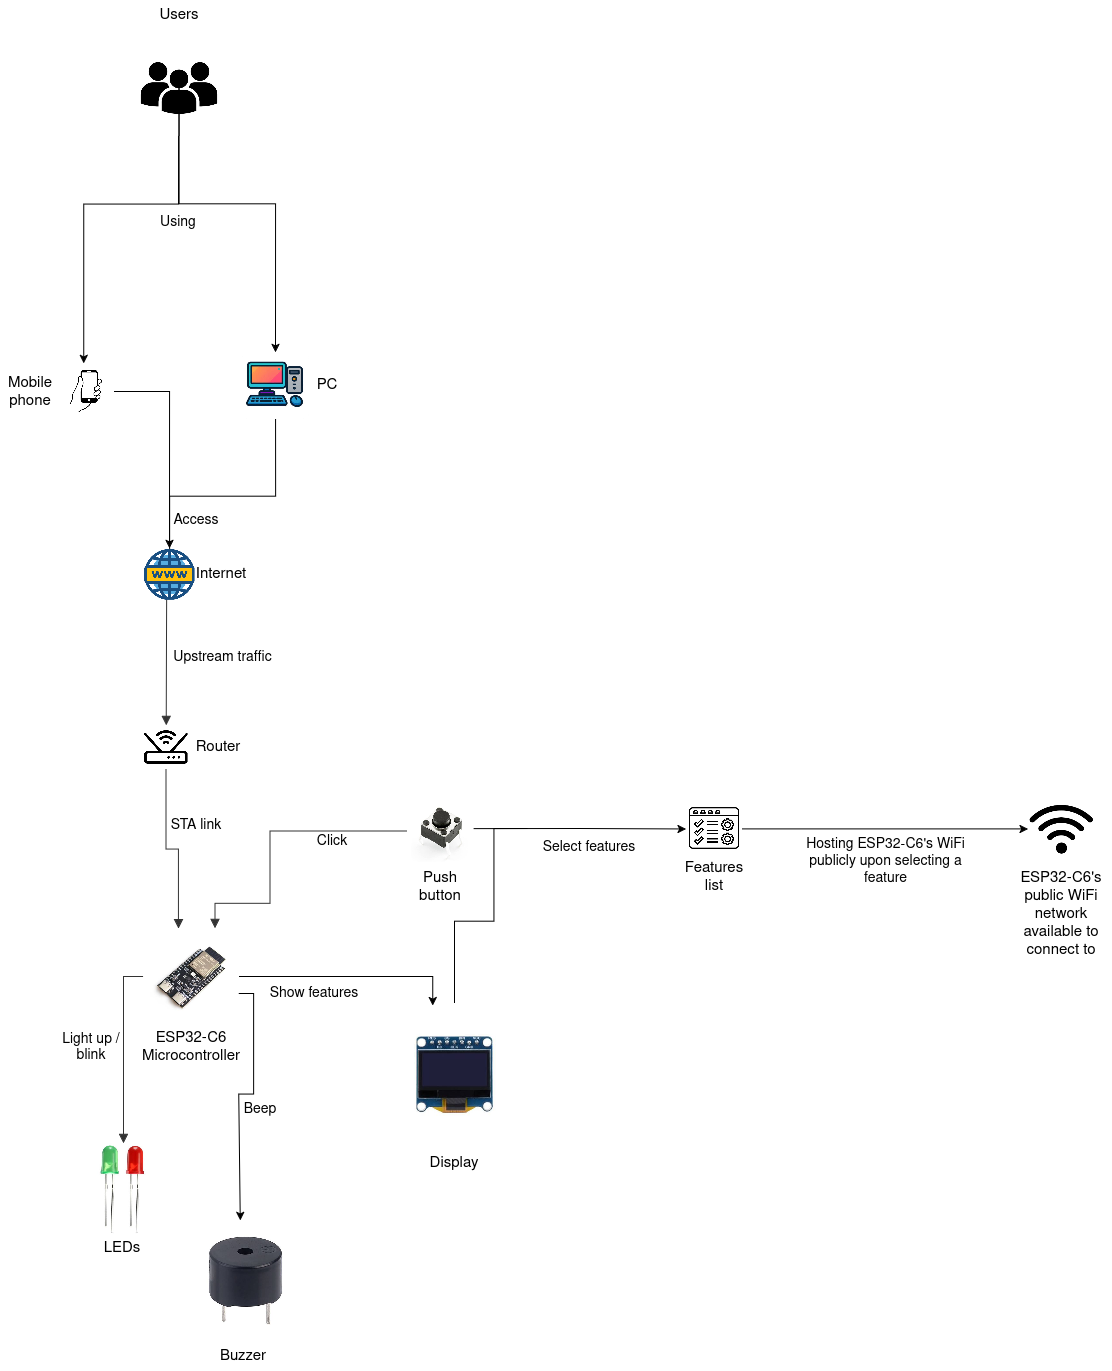
\includegraphics[width=\columnwidth]{system_architecture.png}
  \caption{System architecture.}
  \label{fig:system_architecture}
\end{figure}

\subsection{Hardware Circuit Interfacing}
GPIO pin assignments on the ESP32-C6 \cite{esp32c6} are assigned as follows:
\begin{itemize}
    \item \textbf{Buzzer Output:} GPIO 0
    \item \textbf{Button Input:} GPIO 1
    \item \textbf{Blue Activity LED:} GPIO 2
    \item \textbf{Orange Warning LED:} GPIO 3
    \item \textbf{Addressable RGB LED:} GPIO 8
    \item \textbf{I2C Bus:} GPIO 6 (SDA) and GPIO 7 (SCL)
\end{itemize}

A dedicated $1\,\text{k}\Omega$ resistor connects to each active component (buzzer, push button, Blue LED, and Orange LED) for current limiting and circuit protection. The schematic circuit diagram is shown in Fig.~\ref{fig:circuit_diagram}, and the physical breadboard connection layout is shown in Fig.~\ref{fig:practical_circuit_diagram}. Table~\ref{tab:component_cost_analysis} lists the itemized component costs.

\begin{table}[htbp]
  \centering
  \caption{Hardware Component Cost Analysis}
  \label{tab:component_cost_analysis}
  \small
  \begin{tabularx}{\linewidth}{@{}Xcrr@{}}
    \toprule
    \textbf{Component Name} & \textbf{Ref.} & \textbf{Price (BDT)} & \textbf{Price (USD)} \\
    \midrule
    nanoESP32-C6 Development Board & \cite{rbd_esp32c6} & 950.00 & 7.79 \\
    0.96'' I2C OLED Display Yellow & \cite{rbd_oled} & 260.00 & 2.13 \\
    Passive Buzzer 5V & \cite{rbd_buzzer} & 15.00 & 0.12 \\
    5mm Blue LED (1 pc) & \cite{rbd_blue_led} & 3.00 & 0.02 \\
    5mm Orange LED (1 pc) & \cite{rbd_orange_led} & 3.00 & 0.02 \\
    Push Button Switch (2-PIN, 1 pc) & \cite{rbd_button} & 5.00 & 0.04 \\
    1\,k$\Omega$ 1/4W Resistors (4 pcs) & \cite{rbd_resistor} & 4.00 & 0.03 \\
    Breadboard Half Size (400 Tie Points, 2 pcs) & \cite{rbd_breadboard} & 180.00 & 1.48 \\
    Male to Male Jumper Wires (8 Pcs, 20cm) & \cite{rbd_jumper} & 22.00 & 0.18 \\
    \midrule
    \textbf{Total} & & \textbf{1,442.00} & \textbf{11.82} \\
    \bottomrule
  \end{tabularx}
\end{table}

% Circuit Diagram
\begin{figure}[htbp]
  \centering
  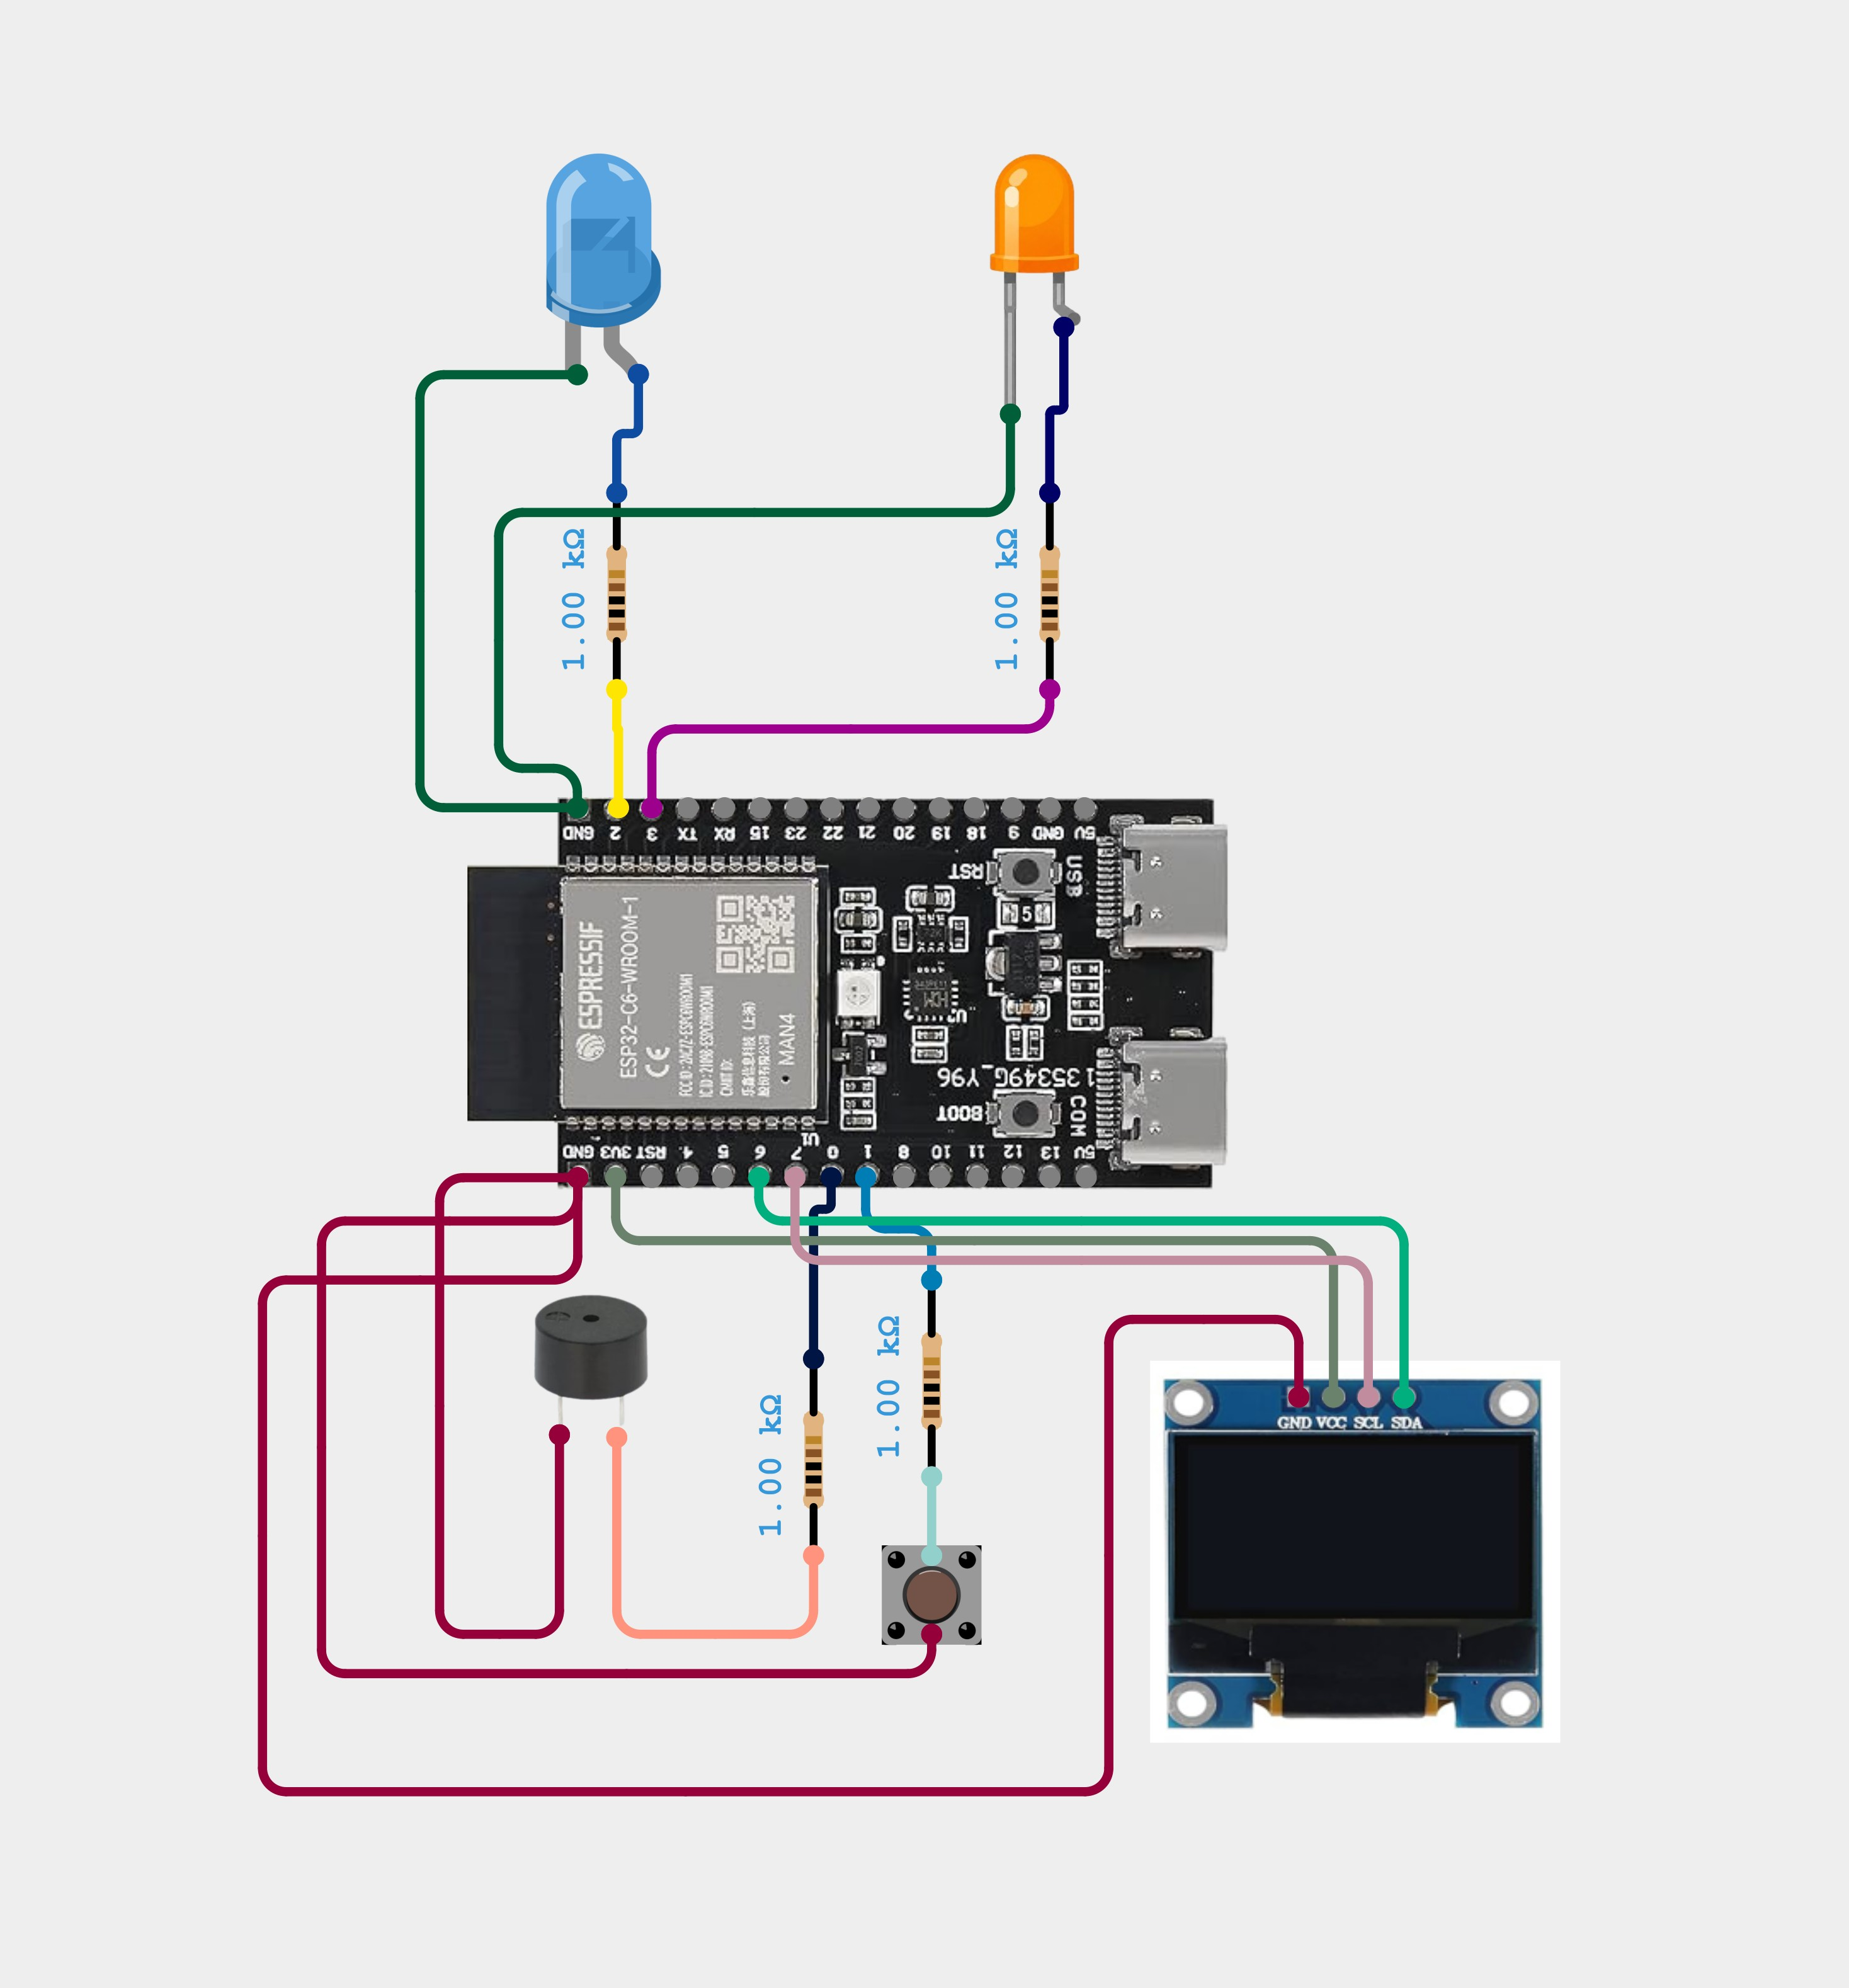
\includegraphics[width=\columnwidth]{circuit_diagram.png}
  \caption{Circuit diagram of the system.}
  \label{fig:circuit_diagram}
\end{figure}

\begin{figure}[htbp]
  \centering
  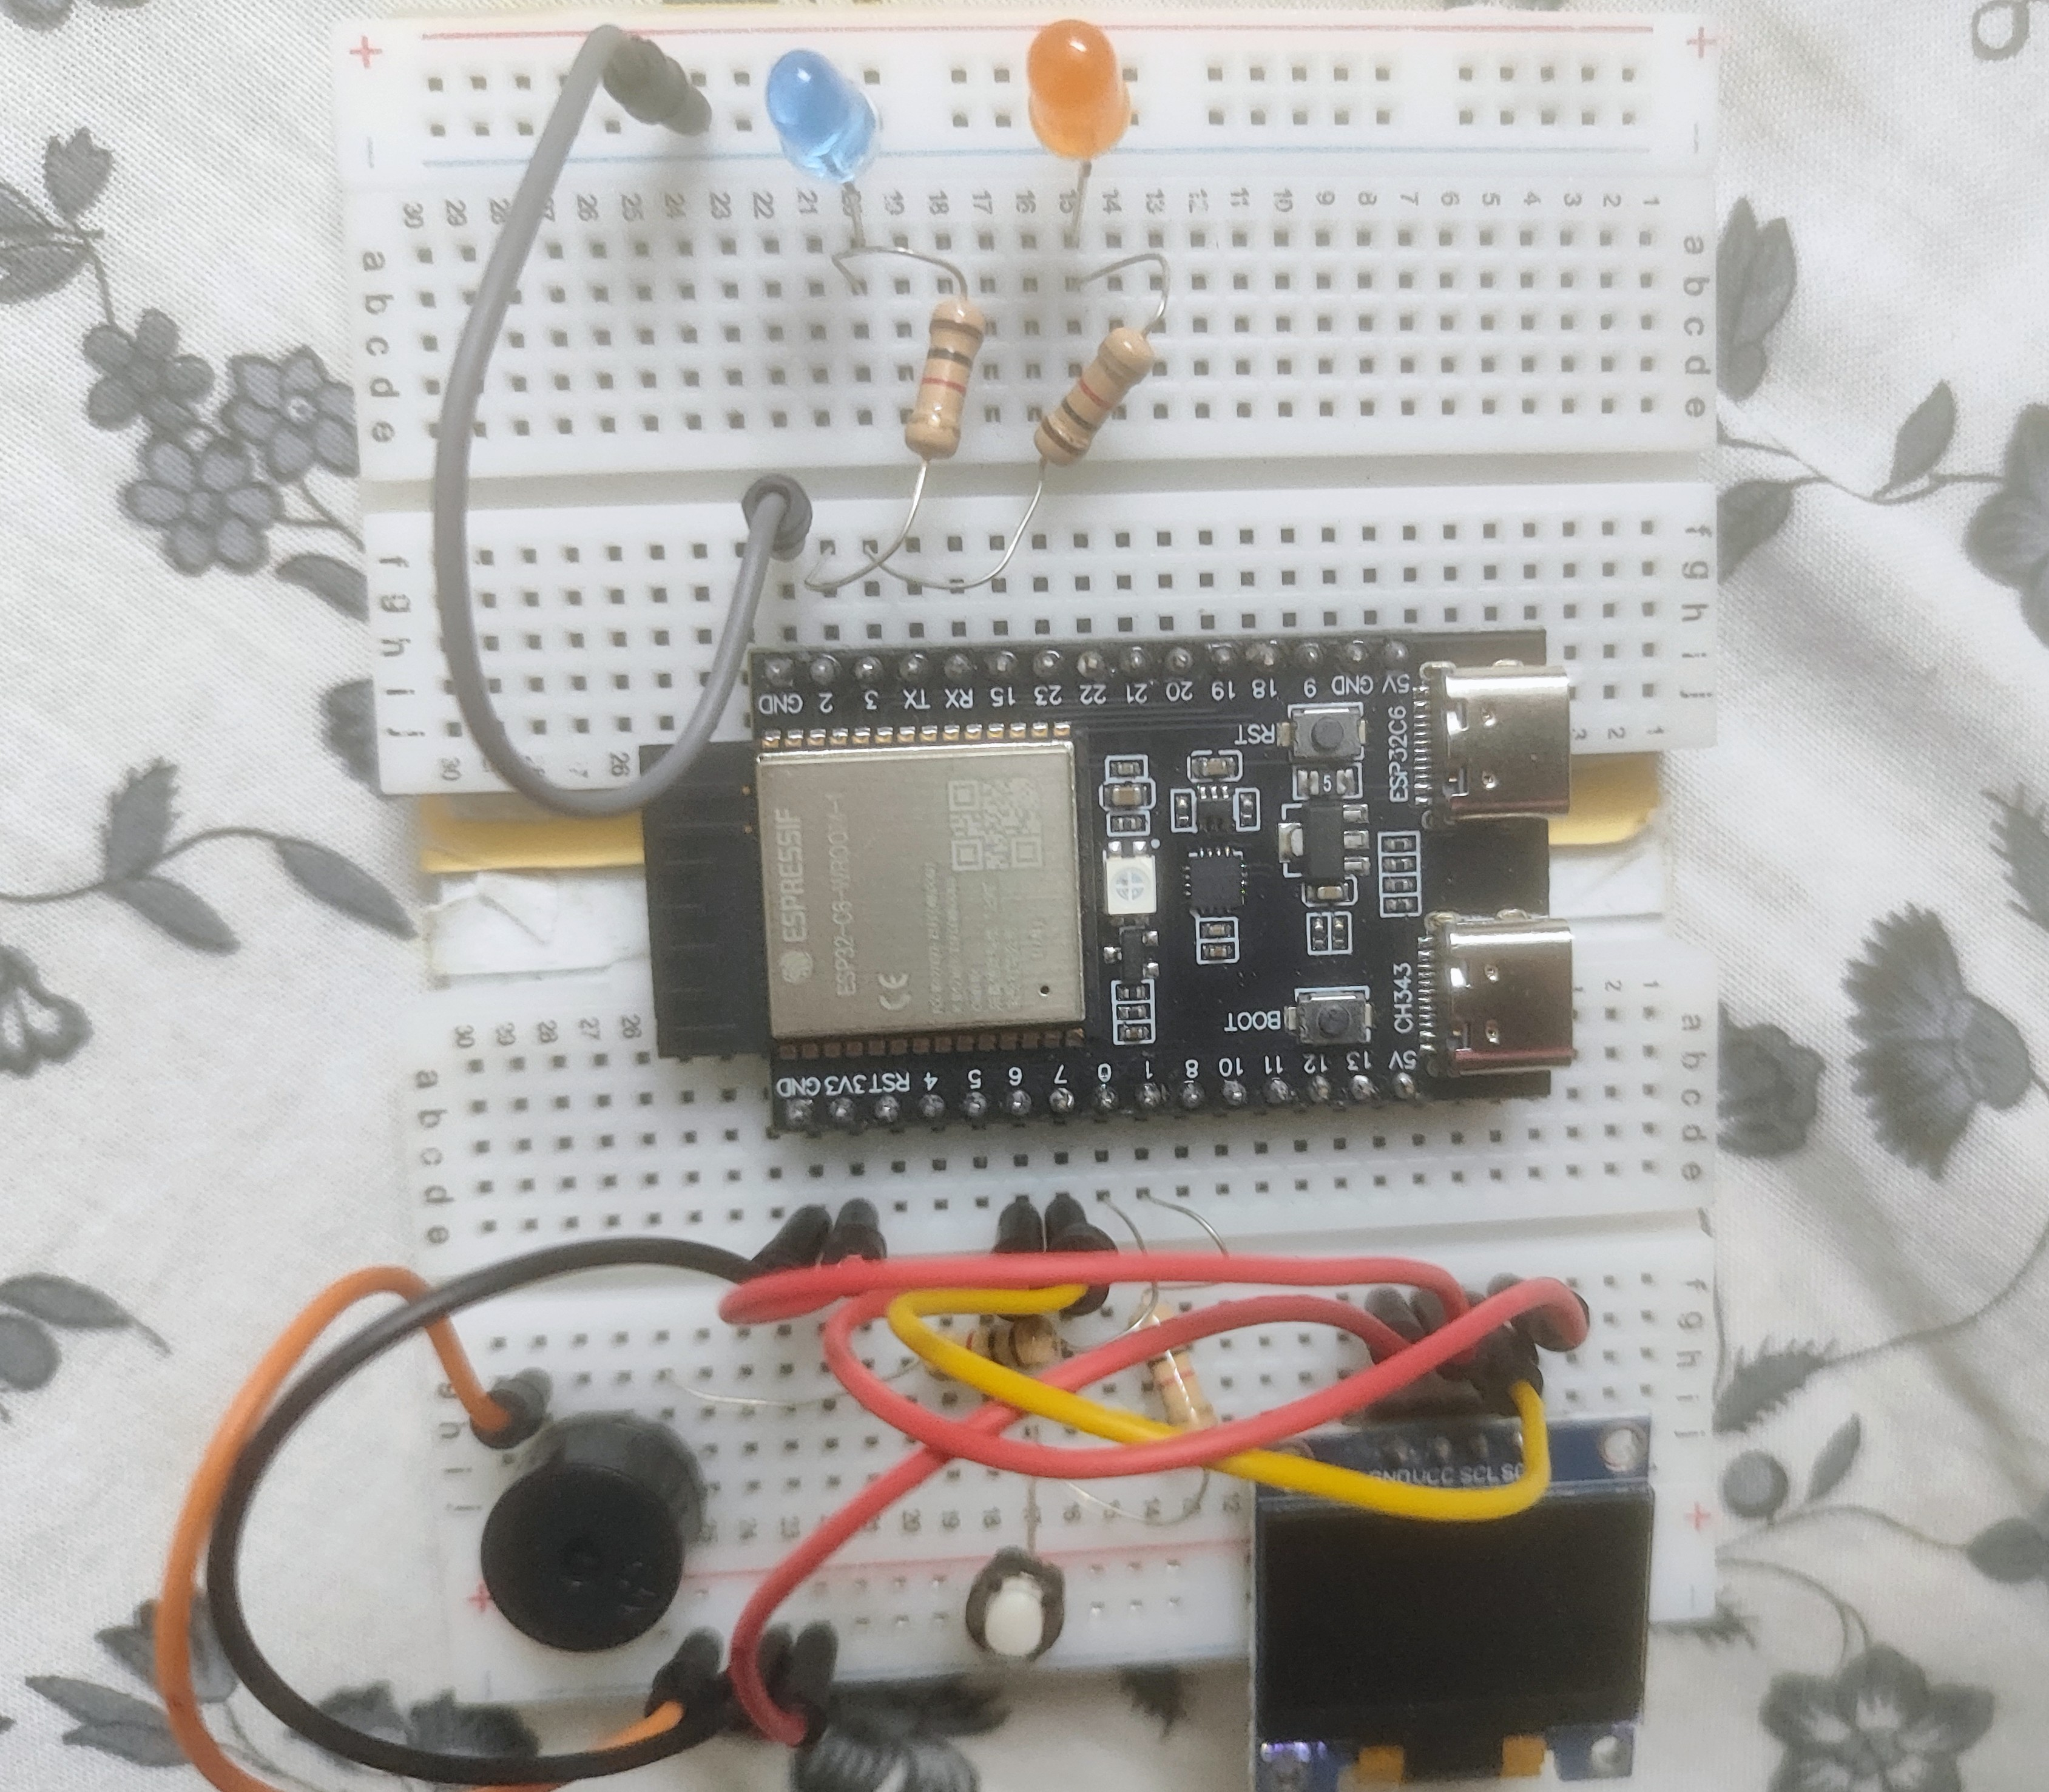
\includegraphics[width=\columnwidth]{practical_circuit_diagram.jpg}
  \caption{Practical circuit diagram of the hardware setup.}
  \label{fig:practical_circuit_diagram}
\end{figure}

\subsection{Software Architecture \& Feature Execution}
The firmware runs a main loop across six operating modes built on the Arduino framework for ESP32 \cite{arduino_esp32}.

\subsubsection{Feature 1: AP Ping Monitor}
Enables promiscuous Wi-Fi mode using \texttt{esp\_wifi\_set\_promiscuous()} \cite{espressif_idf}. The sniffer callback parses incoming 802.11 data frames \cite{ieee80211} and compares destination MAC addresses against the module's SoftAP MAC address. If packet throughput exceeds 10\,pkts/sec, the system turns the RGB LED yellow and sounds a single $2400\,\text{Hz}$ beep.

\subsubsection{Feature 2: AP Data Monitor}
Counts total received packets ($\text{Total Rx}$) and updates every $200\,\text{ms}$. The Blue LED flashes and the RGB LED increases brightness when active packet traffic is detected.

\subsubsection{Feature 3: Client Logger}
Monitors station connection events (\texttt{ARDUINO\_EVENT\_WIFI\_AP\_STACONNECTED}) \cite{arduino_esp32}. When a client joins the SoftAP, the device reads its MAC address, displays it in hexadecimal format on the OLED screen, and plays a $2400\,\text{Hz}$ audio tone.

\subsubsection{Feature 4: Flood Monitor}
Calculates incoming data frame rates per second. If frame rates exceed 100\,pkts/sec, the device flags a traffic flood attack by triggering a $2500\,\text{Hz}$ siren, setting the RGB LED to red, and displaying a warning on the OLED screen.

\subsubsection{Feature 5: Port Scan}
Runs four simultaneous TCP server listeners on common ports: FTP (21), SSH (22), HTTP (80), and HTTPS (443). When an incoming client attempts to connect to any port, the server accepts and immediately closes the socket to conserve memory \cite{honeypot_iot}. Detecting a connection attempt triggers a 3-second alternating siren ($1800\,\text{Hz}$--$2800\,\text{Hz}$) and flashes the RGB LED red-purple.

\begin{table*}[!t]
  \centering
  \caption{Feature and Cost Comparison Against Existing Platforms}
  \label{tab:product_comparison}
  \small
  \begin{tabular}{lcccc}
    \toprule
    \textbf{Feature} & \textbf{This Work (Rogue Wi-Fi AP Detector)} & \textbf{ESP32 Marauder \cite{marauder}} & \textbf{WiFi Pineapple Mark VII \cite{pineapple}} \\
    \midrule
    Approximate Cost (USD) & \$10 & \$102 & \$250 \\
    Bare-Metal (No OS) & Yes & Yes & No (Linux) \\
    Cold Boot Time & $<1\,\text{s}$ & $<1\,\text{s}$ & $\sim$45\,s \\
    Rogue AP Detection & Yes & Yes & Yes \\
    DoS / Flood Alarm & Yes & Yes & Yes \\
    Multi-Port TCP Honeypot & Yes & No & No \\
    Layer-3 NAPT Range Extender & Yes & No & No \\
    Automatic RSSI AP Selection & Yes & No & No \\
    Onboard Acoustic Siren & Yes & No & No \\
    Onboard Visual Displays & Yes (OLED + RGB LED) & Yes (Display) & Limited (Single LED) \\
    \bottomrule
  \end{tabular}
\end{table*}

\subsubsection{Feature 6: NAPT Wi-Fi Repeater}
Runs in dual AP+STA mode (\texttt{WIFI\_AP\_STA}) \cite{espressif_idf}. The user can connect to a pre-configured target SSID or scan for open networks. In open scan mode, the system scans surrounding networks, selects the open AP with the strongest signal strength (RSSI), and connects to it.

After connecting to the upstream network, the firmware enables Layer-3 NAPT in the LwIP stack \cite{lwip}:
\begin{equation}
\mathtt{ip\_napt\_enable}\left(\mathtt{softAP\_IP}, 1\right)
\end{equation}
Enabling NAPT uses \texttt{LOCK\_TCPIP\_CORE()} and \texttt{UNLOCK\_TCPIP\_CORE()} macros \cite{lwip} to ensure thread safety while forwarding packets. The SoftAP DHCP server then passes the upstream DNS server address to connected clients, defaulting to Google DNS ($8.8.8.8$) if no upstream DNS is available \cite{napt_ref}.

\FloatBarrier
\section{Result Analysis}
The complete hardware prototype operating under test conditions is shown in Fig.~\ref{fig:working_prototype}. System performance metrics and response times across all six operating modes were recorded using serial monitor logs, as summarized in Table~\ref{tab:results}.

\begin{figure}[htbp]
  \centering
  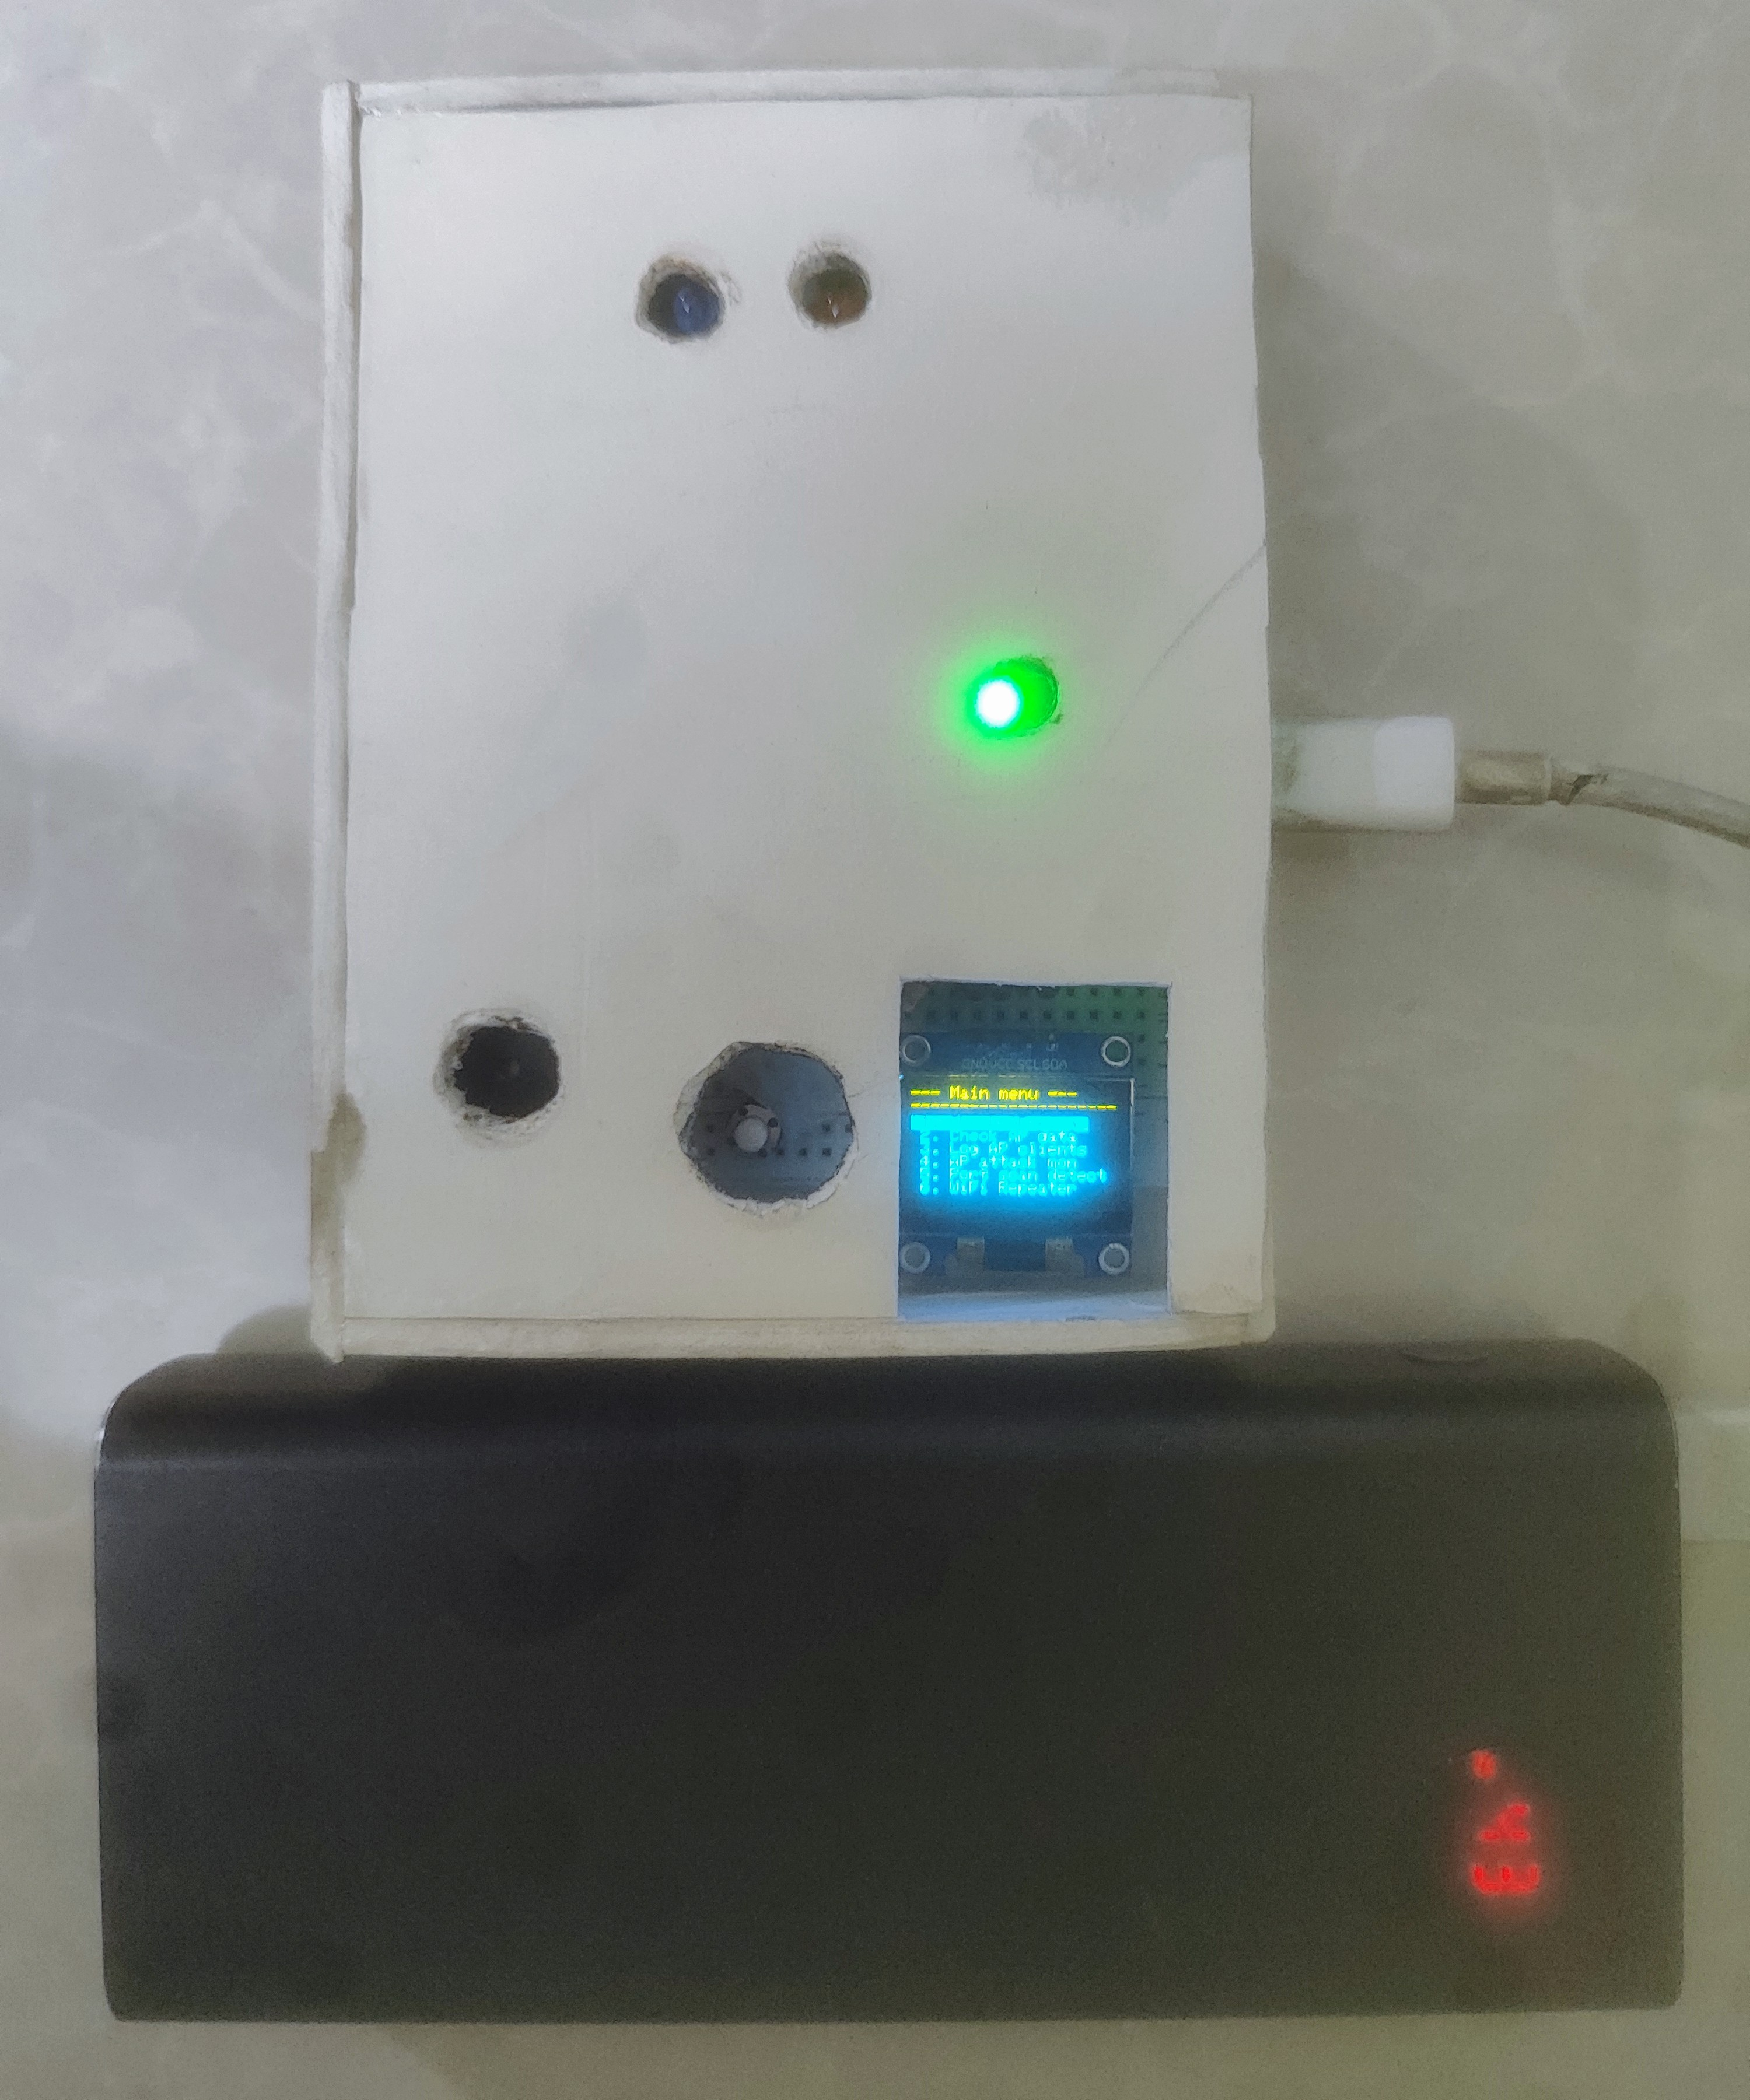
\includegraphics[width=\columnwidth]{working_prototype.jpg}
  \caption{Working prototype of the Rogue Wi-Fi AP Detector.}
  \label{fig:working_prototype}
\end{figure}

\begin{table}[htbp]
\caption{System Performance Results from Serial Monitor Testing}
\label{tab:results}
\centering
\small
\begin{tabularx}{\linewidth}{@{}lXX@{}}
\toprule
\textbf{Feature Mode} & \textbf{Metric / Parameter} & \textbf{Value} \\
\midrule
AP Ping Monitor (F1) & Target Frame Processing Latency & $11.8\,\text{ms}$ \\
AP Ping Monitor (F1) & Trigger Warning Threshold & $> 10\,\text{pkts/sec}$ \\
AP Data Monitor (F2) & Serial telemetry refresh interval & $200\,\text{ms}$ \\
Client Logger (F3) & Station MAC Parsing Latency & $14.2\,\text{ms}$ \\
Flood Monitor (F4) & Attack Alarm Trigger Threshold & $> 100\,\text{pkts/sec}$ \\
Flood Monitor (F4) & Alert Audio Activation Delay & $< 4.5\,\text{ms}$ \\
Port Scan (F5) & Connection Flush \& Termination & $2.1\,\text{ms}$ \\
Port Scan (F5) & Multi-Port Polling Loop Overhead & $0.35\,\text{ms}$ \\
WiFi Repeater (F6) & Open AP Scan Target Acquisition & $4.613\,\text{s}$ \\
WiFi Repeater (F6) & Layer-3 Forwarding Init Time & $< 1\,\text{ms}$ \\
WiFi Repeater (F6) & Connection Timeout Fallback & $15.0\,\text{s}$ (configured) \\
\bottomrule
\end{tabularx}
\end{table}

Promiscuous frame capture processed 802.11 packet headers \cite{ieee80211} without memory crashes or system freezes. DoS flood testing for Feature 4 (Flood Monitor) was conducted using the PingTools app \cite{pingtools} on Android by sending rapid traffic to the SoftAP; packet rates above $100\,\text{pkts/sec}$ consistently activated the alarm siren. Feature 5 (Port Scan) was verified by scanning ports 21, 22, 80, and 443 with PingTools; connection attempts were detected and triggered the siren in under $3\,\text{ms}$ without interrupting the main loop.

Feature 6 (Wi-Fi Repeater) scanned and connected to the strongest open access point (RSSI $-30\,\text{dBm}$) in $4.613\,\text{s}$. Layer-3 NAPT setup and DHCP/DNS configuration completed in under $1\,\text{ms}$. Using \texttt{LOCK\_TCPIP\_CORE()} prevented memory crashes during DNS configuration changes \cite{lwip}.

\FloatBarrier
\section{Challenges Faced}
Developing and testing the unified firmware on the ESP32-C6 presented five practical challenges:

\begin{enumerate}
    \item \textbf{Hardware Serial Debugging vs. Native USB CDC:} Serial debug output failed to stream on boot because native USB CDC conflicted with the hardware UART peripheral \cite{espressif_idf}. Disabling USB CDC on Boot in Arduino IDE settings routed \texttt{Serial.print()} over hardware UART, restoring serial logs.
    \item \textbf{Wi-Fi Stack Mode Transitions:} Switching directly between AP mode (\texttt{WIFI\_AP}) and repeater mode (\texttt{WIFI\_AP\_STA}) corrupted internal Wi-Fi driver state \cite{espressif_idf}. Calling \texttt{WiFi.mode(WIFI\_OFF)} to reset the Wi-Fi state before changing modes resolved the issue.
    \item \textbf{LwIP Thread Safety \& Core Locking:} Enabling NAPT via \texttt{ip\_napt\_enable()} while client data was passing caused memory crashes \cite{lwip}. Using \texttt{LOCK\_TCPIP\_CORE()} and \texttt{UNLOCK\_TCPIP\_CORE()} during NAPT setup solved the problem.
    \item \textbf{Non-Blocking Multi-Peripheral Execution:} Playing buzzer tones, updating the OLED display, reading button clicks, and checking honeypot ports needed to run without using \texttt{delay()}. A timer mechanism using \texttt{millis()} with interval counters allowed all tasks to run smoothly together.
    \item \textbf{Indicator Component Substitution:} Red and green status LEDs were originally planned for status and alert signals. Local store availability required substituting 5mm blue and orange LEDs \cite{rbd_blue_led}, \cite{rbd_orange_led}.
\end{enumerate}

\FloatBarrier
\section{Conclusion}
The Rogue Wi-Fi Access Point Detector combines Wi-Fi security monitoring, TCP honeypots, and Layer-3 network repeating on an ESP32-C6 RISC-V microcontroller at a hardware cost under 12\,USD. The non-blocking firmware allows packet sniffing, flood detection, honeypot alerts, and NAPT repeating to run reliably on a low-power device. Future work includes adding Bluetooth Low Energy (BLE) attack monitoring, battery power management, and cloud logging over MQTT.

\FloatBarrier
\begin{thebibliography}{00}
\bibitem{esp32c6}
Espressif Systems, ``ESP32-C6 Series Datasheet,'' Rev.~1.1, Espressif Systems, Shanghai, 2023. [Online]. Available: \url{https://www.espressif.com/sites/default/files/documentation/esp32-c6_datasheet_en.pdf}

\bibitem{ieee80211}
IEEE Computer Society, ``IEEE Standard for Information Technology---Telecommunications and Information Exchange Between Systems---Local and Metropolitan Area Networks---Specific Requirements---Part 11: Wireless LAN Medium Access Control (MAC) and Physical Layer (PHY) Specifications,'' \textit{IEEE Std 802.11-2020}, Feb.~2021, doi: 10.1109/IEEESTD.2021.9363693.

\bibitem{lwip}
A. Dunkels, ``Full TCP/IP for 8-Bit Architectures,'' in \textit{Proc. 1st Int. Conf. Embedded Networked Sensor Systems (SenSys)}, Los Angeles, CA, USA, Nov. 2003, pp. 85--98, doi: 10.1145/958491.958502.

\bibitem{honeypot_iot}
S. Dowling, M. Schukat, and E. Higgins, ``A ZigBee Honeypot to Assess IoT Cyberattack Behaviour,'' in \textit{Proc. 28th Irish Signals and Systems Conf. (ISSC)}, Killarney, Ireland, Jun. 2017, pp. 1--6, doi: 10.1109/ISSC.2017.7983624.

\bibitem{napt_ref}
P. Srisuresh and K. Egevang, ``Traditional IP Network Address Translator (Traditional NAT),'' IETF RFC 3022, Jan. 2001. [Online]. Available: \url{https://www.rfc-editor.org/rfc/rfc3022}

\bibitem{espressif_idf}
Espressif Systems, ``ESP-IDF Programming Guide,'' v5.x, Espressif Systems, 2024. [Online]. Available: \url{https://docs.espressif.com/projects/esp-idf/en/latest/}

\bibitem{arduino_esp32}
Espressif Systems, ``Arduino Core for ESP32,'' GitHub repository, 2024. [Online]. Available: \url{https://github.com/espressif/arduino-esp32}

\bibitem{ssd1306}
Adafruit Industries, ``Adafruit SSD1306 OLED Driver Library,'' GitHub repository, 2024. [Online]. Available: \url{https://github.com/adafruit/Adafruit_SSD1306}

\bibitem{neopixel}
Adafruit Industries, ``Adafruit NeoPixel Library,'' GitHub repository, 2024. [Online]. Available: \url{https://github.com/adafruit/Adafruit_NeoPixel}

\bibitem{marauder}
J. Betterton, ``ESP32 Marauder: A Suite of WiFi/Bluetooth Offensive and Defensive Tools for the ESP32,'' GitHub repository, 2024. [Online]. Available: \url{https://github.com/justcallmekoko/ESP32Marauder}

\bibitem{pineapple}
Hak5 LLC, ``WiFi Pineapple Mark VII User Guide,'' Hak5 Documentation, 2023. [Online]. Available: \url{https://docs.hak5.org/wifi-pineapple}

\bibitem{pingtools}
StreamSoft, ``PingTools Network Utilities,'' Google Play Store, 2024. [Online]. Available: \url{https://play.google.com/store/apps/details?id=ua.com.streamsoft.pingtools}

\bibitem{rbd_esp32c6}
RoboticsBD, ``nanoESP32-C6 Development Board Minimum System Board ESP32 Core Board RISC-V Espressif IoT,'' \textit{RoboticsBD Store}, 2024. [Online]. Available: \url{https://store.roboticsbd.com/internet-of-things-iot/2768-nanoesp32-c6-development-board-minimum-system-board-esp32-core-board-risc-v-espressif-iot-robotics-bangladesh.html}

\bibitem{rbd_oled}
RoboticsBD, ``0.96 Inch I2C OLED Display Yellow,'' \textit{RoboticsBD Store}, 2024. [Online]. Available: \url{https://store.roboticsbd.com/arduino-shield/353-096-inch-i2c-oled-display-yellow-robotics-bangladesh.html}

\bibitem{rbd_buzzer}
RoboticsBD, ``Passive Buzzer 5V,'' \textit{RoboticsBD Store}, 2024. [Online]. Available: \url{https://store.roboticsbd.com/components/767-passive-buzzer-5v-robotics-bangladesh.html}

\bibitem{rbd_blue_led}
RoboticsBD, ``5mm Blue LED - Pack of 5,'' \textit{RoboticsBD Store}, 2024. [Online]. Available: \url{https://store.roboticsbd.com/led/1300-blue-led-5mmpack-of-5-robotics-bangladesh.html}

\bibitem{rbd_orange_led}
RoboticsBD, ``5mm Orange LED,'' \textit{RoboticsBD Store}, 2024. [Online]. Available: \url{https://store.roboticsbd.com/led/874-5-mm-orange-led-robotics-bangladesh.html}

\bibitem{rbd_button}
RoboticsBD, ``Push Button Switch (2PIN),'' \textit{RoboticsBD Store}, 2024. [Online]. Available: \url{https://store.roboticsbd.com/electronic-switches/761-push-button-switch-robotics-bangladesh.html}

\bibitem{rbd_resistor}
RoboticsBD, ``Kiloohm (K$\Omega$) 1/4W Resistors - Pack of 5,'' \textit{RoboticsBD Store}, 2024. [Online]. Available: \url{https://store.roboticsbd.com/components/245-41-resistor-robotics-bangladesh.html}

\bibitem{rbd_breadboard}
RoboticsBD, ``Breadboard Half Size Bare 400 Tie Points,'' \textit{RoboticsBD Store}, 2024. [Online]. Available: \url{https://store.roboticsbd.com/robotics-parts/120-breadboard-half-size-bare-400-tie-points-robotics-bangladesh.html}

\bibitem{rbd_jumper}
RoboticsBD, ``Male to Male Jumper Wires 20 Pcs 20cm,'' \textit{RoboticsBD Store}, 2024. [Online]. Available: \url{https://store.roboticsbd.com/cables-wire/2639-male-to-male-jumper-wires-20-pcs-20cm-robotics-bangladesh.html}
\end{thebibliography}

\end{document}
